% ============================================================
%  D flip-flop - block symbol (with edge-trigger clock notation).
%  Compile:  pdflatex symbol.tex
% ============================================================
\documentclass[border=14pt]{standalone}
\usepackage{tikz}
\usepackage{amsmath}
\begin{document}
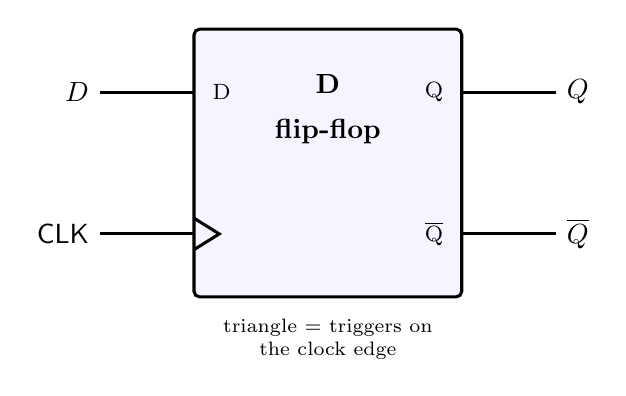
\begin{tikzpicture}[line width=1.1pt, font=\sffamily]
  \draw[rounded corners=2pt, fill=blue!4] (0,0) rectangle (3.4,3.4);
  \node[font=\bfseries] at (1.7,2.7) {D};
  \node[font=\bfseries] at (1.7,2.1) {flip-flop};
  % D input
  \draw (-1.2,2.6) node[left]{$D$} -- (0,2.6);
  \node[anchor=west,font=\footnotesize] at (0.1,2.6) {D};
  % clock input with edge-trigger triangle
  \draw (-1.2,0.8) node[left]{CLK} -- (0,0.8);
  \draw (0,0.6) -- (0.32,0.8) -- (0,1.0);      % > edge-trigger marker
  % outputs
  \draw (3.4,2.6) -- (4.6,2.6) node[right]{$Q$};
  \draw (3.4,0.8) -- (4.6,0.8) node[right]{$\overline{Q}$};
  \node[anchor=east,font=\footnotesize] at (3.3,2.6) {Q};
  \node[anchor=east,font=\footnotesize] at (3.3,0.8) {$\overline{\mathrm Q}$};
  \node[font=\scriptsize,anchor=north,align=center] at (1.7,-0.15) {triangle = triggers on\\the clock edge};
\end{tikzpicture}
\end{document}
